% fig5c-transform-sheaf.tex
\documentclass[tikz,border=12pt]{standalone}
% common-styles.tex
% Shared TikZ styles for wonton-proof paper figures

\usepackage{silence}
\WarningFilter{latex}{Missing character} 
\tracinglostchars=0 % Suppress engine-level "Missing character" warnings

\usepackage{fontspec}
\usepackage{unicode-math}

% Use filenames for reliability with Tectonic
\setmainfont{LibertinusSerif-Regular.otf}[
    BoldFont=LibertinusSerif-Bold.otf,
    ItalicFont=LibertinusSerif-Italic.otf,
    BoldItalicFont=LibertinusSerif-BoldItalic.otf
]
\setsansfont{LibertinusSans-Regular.otf}[
    BoldFont=LibertinusSans-Bold.otf,
    ItalicFont=LibertinusSans-Italic.otf
]
\setmonofont{LibertinusMono-Regular.otf}

% Try a more standard math font if LibertinusMath is causing nullfont issues
\setmathfont{LibertinusMath-Regular.otf}
% \setmathfont{latinmodern-math.otf}[range=digits] 

\usepackage{amsmath}
\usepackage{tikz}
\usepackage{forest}

\usetikzlibrary{
    arrows.meta,
    calc,
    decorations.pathreplacing,
    fit,
    positioning,
    shapes.geometric,
    shapes.misc,
    backgrounds,
    shadows.blur,
    fadings
}

% Color palette (muted, print-friendly)
\definecolor{ink}{RGB}{45,45,52}
\definecolor{muted}{RGB}{115,115,125}
\definecolor{highlight}{RGB}{198,120,44}
\definecolor{accentblue}{RGB}{86,130,178}
\definecolor{accentgreen}{RGB}{84,156,132}
\definecolor{blocked}{RGB}{140,75,75}
\definecolor{goalnode}{RGB}{255,255,255}
\definecolor{terminal}{RGB}{238,239,244}
\definecolor{deadnode}{RGB}{248,245,245}
\definecolor{flowbox}{RGB}{250,250,252}
\definecolor{basin1}{RGB}{224,234,248}
\definecolor{basin2}{RGB}{246,232,221}
\definecolor{basin3}{RGB}{228,242,234}
\definecolor{heatbase}{RGB}{86,130,178}

\tikzset{
    line cap=round,
    line join=round,
    pop/.style={
        blur shadow={shadow blur steps=5, shadow blur extra rounding=1.3pt}
    },
    base node/.style={
        rounded rectangle,
        draw=ink,
        line width=0.6pt,
        fill=goalnode,
        text=ink,
        minimum width=2.2cm,
        minimum height=0.7cm,
        align=center,
        pop
    },
    goal/.style={base node, fill=goalnode},
    terminal/.style={base node, fill=terminal, line width=0.9pt},
    dead/.style={base node, fill=deadnode, dashed},
    flowbox/.style={
        rectangle,
        draw=muted,
        rounded corners=3pt,
        fill=flowbox,
        minimum width=1.8cm,
        minimum height=0.6cm,
        align=center,
        font=\normalfont\small,
        text=ink,
        pop
    },
    decision/.style={
        diamond,
        draw=muted,
        fill=flowbox,
        aspect=2.4,
        font=\normalfont\small,
        inner sep=1pt,
        text=ink
    },
    protocolbox/.style={
        rectangle,
        draw=muted,
        rounded corners=4pt,
        fill=flowbox,
        minimum width=2cm,
        minimum height=0.8cm,
        font=\normalfont\small,
        align=center,
        text=ink
    },
    tactic/.style={
        ->,
        >=Stealth,
        draw=muted,
        line width=0.75pt
    },
    tacticlight/.style={
        ->,
        >=Stealth,
        draw=muted!45,
        dashed,
        line width=0.6pt
    },
    backprop/.style={
        ->,
        >=Stealth,
        draw=muted!70,
        dashed,
        line width=0.6pt
    },
    selected/.style={
        tactic,
        draw=highlight,
        line width=1.4pt
    },
    divergetactic/.style={
        tactic,
        draw=highlight,
        line width=1.4pt
    },
    divergenode/.style={
        base node,
        draw=highlight,
        line width=1.0pt
    },
    divergeblock/.style={
        blockedtactic,
        line width=1.2pt
    },
    blockedtactic/.style={
        tactic,
        draw=blocked,
        densely dashed
    },
    flowarrow/.style={
        ->,
        >=Stealth,
        draw=muted,
        line width=0.75pt
    },
    crosslink/.style={
        -,
        draw=muted!70,
        dotted,
        line width=0.6pt
    },
    annot/.style={
        font=\normalfont\footnotesize,
        text=muted
    },
    visit/.style={
        annot,
        font=\normalfont\scriptsize
    },
    annotbg/.style={
        annot,
        fill=white,
        inner sep=1.5pt
    },
    tacticlabel/.style={
        annot,
        font=\ttfamily\footnotesize,
        text=muted
    },
    formula/.style={
        font=\normalfont\footnotesize,
        draw=muted,
        rounded corners=2pt,
        fill=white,
        inner sep=3pt
    },
    paneltitle/.style={
        font=\normalfont\bfseries,
        text=ink
    },
    trajectory/.style={
        ->,
        draw=muted!70,
        line width=0.6pt
    }
}

\begin{document}
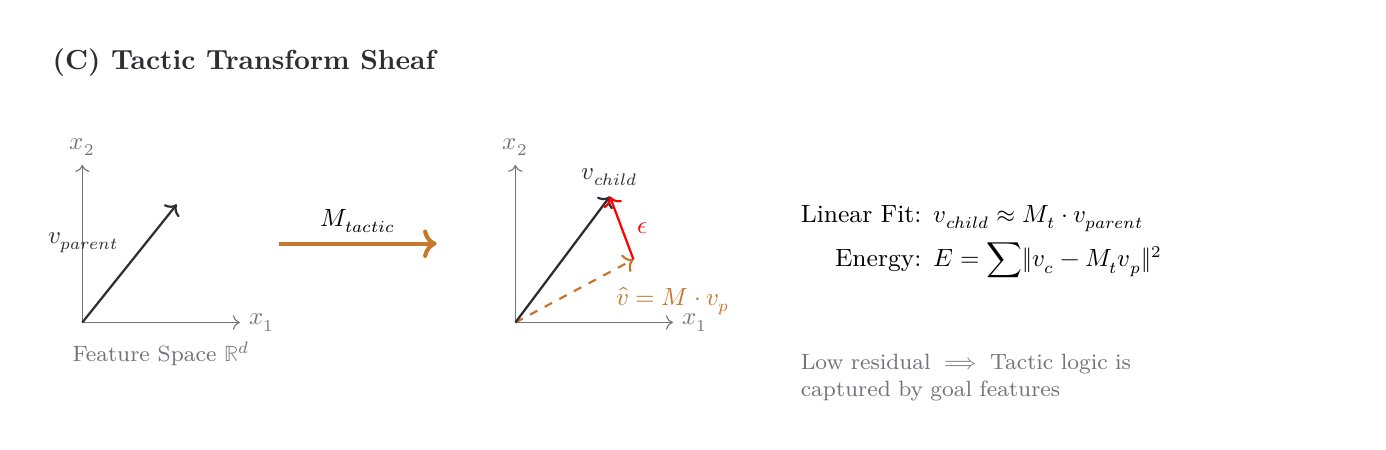
\begin{tikzpicture}[
    every node/.style={font=\small},
    show background rectangle,
    background rectangle/.style={fill=white}
]
\begin{scope}[shift={(0, 0)}]
    \node[paneltitle, anchor=south west] at (-0.5, 3.0) {(C) Tactic Transform Sheaf};
    
    % Parent Feature Space
    \begin{scope}[shift={(0,0)}]
        \draw[->, muted] (0,0) -- (2,0) node[right] {$x_1$};
        \draw[->, muted] (0,0) -- (0,2) node[above] {$x_2$};
        \draw[thick, ink, ->] (0,0) -- (1.2, 1.5) node[midway, above left] {$v_{parent}$};
        \node[annot] at (1.0, -0.4) {Feature Space $\mathbb{R}^d$};
    \end{scope}
    
    % Transformation Arrow
    \draw[->, line width=1.5pt, draw=highlight] (2.5, 1.0) -- (4.5, 1.0) node[midway, above] {$M_{tactic}$};
    
    % Child Feature Space
    \begin{scope}[shift={(5.5,0)}]
        \draw[->, muted] (0,0) -- (2,0) node[right] {$x_1$};
        \draw[->, muted] (0,0) -- (0,2) node[above] {$x_2$};
        
        % Predicted
        \draw[thick, highlight, ->, dashed] (0,0) -- (1.5, 0.8)
            node[pos=0.72, below right, xshift=2pt] {$\hat{v} = M \cdot v_p$};
        
        % Actual
        \draw[thick, ink, ->] (0,0) -- (1.2, 1.6) node[above] {$v_{child}$};
        
        % Residual
        \draw[red, thick, ->] (1.5, 0.8) -- (1.2, 1.6)
            node[midway, right, xshift=2pt] {$\epsilon$};
    \end{scope}
    
    % Matrix Equation
    \node[align=left, text width=6.8cm, anchor=west] at (9.0, 1.05) {
        $\begin{aligned}
            \text{Linear Fit: } & v_{child} \approx M_t \cdot v_{parent} \\
            \text{Energy: } & E = \sum \lVert v_c - M_t v_p\rVert^2
        \end{aligned}$
    };
    
    % Interpretation
    \node[annot, align=left, text width=6.8cm, anchor=west] at (9.0, -0.7) {Low residual $\implies$ Tactic logic is\\captured by goal features};
\end{scope}
\end{tikzpicture}
\end{document}
